\section{Analyzing Algorithms}

\textit{Asymptotic analysis}, or in general, the analysis of function growth, relates heavily to the performance of an algorithm. We can represent algorithms as mathematical functions, and describe their relative performance in terms of the input size. 

\example Consider the linear search algorithm. We know that, in the best case, the item that we are searching for is the first element in the list. In the average case, it is found in the middle of the list. In the worst case, the element does not exist in the list. Because we have to traverse through n elements, namely the n elements of our input list, we say that the linear search grows in linear proportion to its input size. 

\textit{Best-case}, \textit{average-case}, and \textit{worst-case} describe the potential inputs to a function. We can ascribe the same meanings to binary search, the sorting algorithms from the previous chapter, and beyond. Though, we need a notation to denote the growth rate of a function. In computer science we most often make use of Big-Oh notation, which denotes a function's upper bound. That is, a function $f(n) = \mathcal{O}(g(n))$ if, at some point, $f(n)$ begins to forever grow slower than or equal to $g(n)$. We can roughly replace the equals `$=$' sign with a less-than-or-equal-to `$\leq$' sign. One detail to note is that the end-behavior of a polynomial is determined by its highest-order term. For example, $f(n) = 0.5x^2 + 0.5\cos(\textsf{deg}(5x))$ is upper-bounded by $g(n) = 0.5x^2$, because the cosine function is upper-bounded by $1$. Thus, when describing a function in asymptotic terms, we can drop/ignore all coefficients and lower-order terms.

\example Consider the following functions $f(n) = 0.5x^2 + 0.5\cos(\textsf{deg}(5x))$ and $g(n) = 0.2x^3 + 0.3\sin({\textsf{deg}(4x)})$. As we stated, we can drop all lower-order terms and coefficients, meaning $f(n) = n^2$ and $g(n) = n^3$. From here, it is trivial to see that for any $n > 1$, $g(n)$ grows faster than $f(n)$ Thus, we say that $f(n) = \mathcal{O}(g(n))$.\footnote{There is a bit more to the formalism of Big-Oh, but we will explain those details in due time.}
\begin{figure}[H]
  \centering
  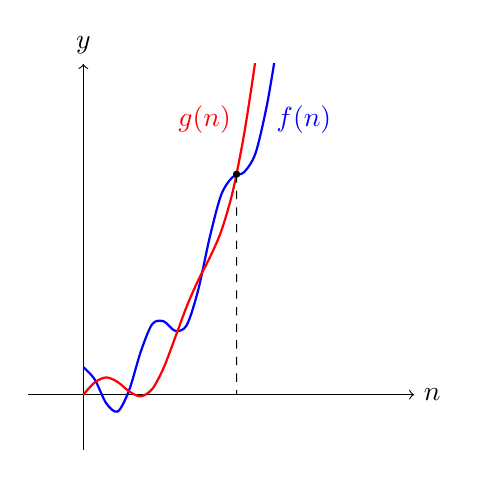
\begin{tikzpicture}[scale=0.7]
      % Axes
      \draw[->] (-1,0) -- (6,0) node[right] {$n$};
      \draw[->] (0,-1) -- (0,6) node[above] {$y$};
  
      \begin{scope}
      \clip (-1,-1) rectangle (5,6);
      % Function g(n)
      \draw[domain=0:5, smooth, thick, blue] plot (\x, {0.5*\x^2 + 0.5*cos(deg(5*\x))});
      \node[blue] at (4,5) {$f(n)$};
      
      % Function f(n)
      \draw[domain=0:5, smooth, thick, red] plot (\x, {0.2*\x^3 + 0.3*sin(deg(4*\x))});
      \node[red] at (2.2,5) {$g(n)$};
      \end{scope}
      % Big-Oh notation
      \coordinate (intersection) at (2.78, 4.0);
      \fill[black] (intersection) circle (1.9pt);
      \draw[dashed] (intersection) -- (2.78,0);
  \end{tikzpicture}
  \caption{$f(n) = \mathcal{O}(g(n))$}
  \end{figure}

There are two other common notations for asymptotic analysis: Big-Omega and Theta. Big-Omega describes the lower-bound of a function, and Theta describes the tight bound of a function. That is, $f(n) = \Omega(g(n))$ if there is a point at which $f(n)$ begins to grow faster than or equal to $g(n)$. We can roughly replace the equals `$=$' sign with a greater-than-or-equal-to `$\geq$' sign. Similarly, $f(n) = \Theta(g(n))$ if $f(n) = \mathcal{O}(g(n))$ and $f(n) = \Omega(g(n))$. We can roughly replace the equals `$=$' sign with an equivalence `$\equiv$' sign. Examples for Omega and Theta are harder to come by without a formalized definition, so we will defer them until later.

\begin{figure}[H]
  \centering
  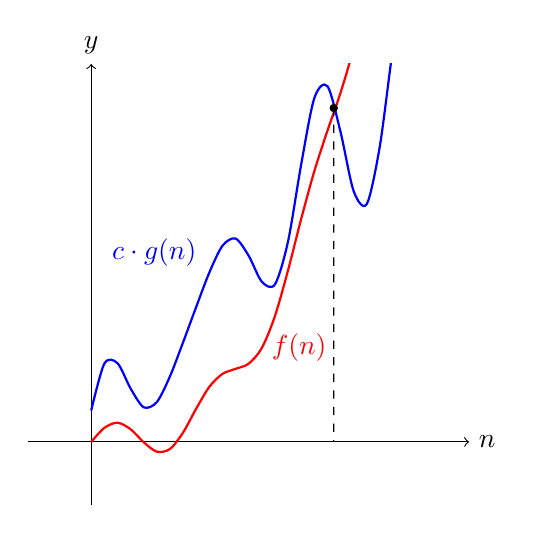
\begin{tikzpicture}[scale=0.8]
    % Axes
    \draw[->] (-1,0) -- (6,0) node[right] {$n$};
    \draw[->] (0,-1) -- (0,6) node[above] {$y$};

    \begin{scope}
    \clip (-1,-1) rectangle (5,6);
    % Function g(n)
    \draw[domain=0:5, smooth, thick, blue] plot (\x, {1.2*\x + 0.5*cos(deg(5*\x)) + sin(deg(4*\x))});
    \node[blue] at (1,3) {$c\cdot{}g(n)$};
    
    % Function f(n)
    \draw[domain=0:5, smooth, thick, red] plot (\x, {0.09*\x^3 + 0.3*sin(deg(4*\x))});
    \node[red] at (3.3, 1.5) {$f(n)$};
    \end{scope}
    % Big-Oh notation
    \coordinate (intersection) at (3.85, 5.3);
    \fill[black] (intersection) circle (1.9pt);
    \draw[dashed] (intersection) -- (3.85,0);
\end{tikzpicture}
\caption{$f(n) = \Omega(g(n))$}
\end{figure}

\begin{figure}[H]
  \centering
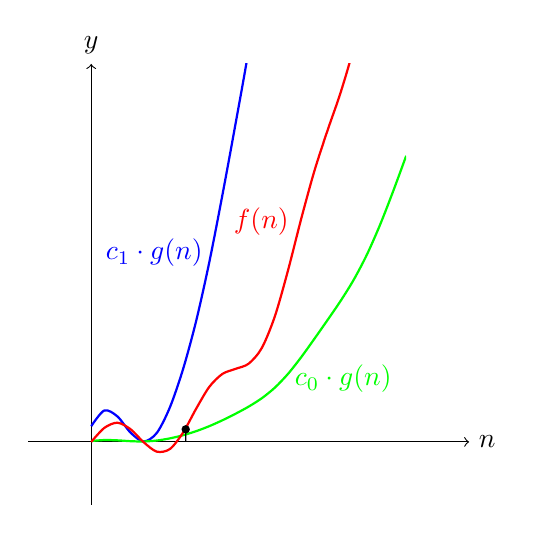
\begin{tikzpicture}[scale=0.8]
  % Axes
  \draw[->] (-1,0) -- (6,0) node[right] {$n$};
  \draw[->] (0,-1) -- (0,6) node[above] {$y$};

  \begin{scope}
  \clip (-1,-1) rectangle (5,6);
  % Function g(n)
  \draw[domain=0:5, smooth, thick, blue] plot (\x, {0.5*(0.8*\x^3 + 0.5*cos(deg(5*\x)) + sin(deg(4*\x))});
  \node[blue] at (1,3) {$c_1\cdot{}g(n)$};

  \draw[domain=0:5, smooth, thick, green] plot (\x, {0.03*(1.2*\x^3 + 0.5*cos(deg(5*\x)) + sin(deg(4*\x))});
  \node[green] at (4,1) {$c_0\cdot{}g(n)$};
  
  % Function f(n)
  \draw[domain=0:5, smooth, thick, red] plot (\x, {0.09*\x^3 + 0.3*sin(deg(4*\x))});
  \node[red] at (2.7, 3.5) {$f(n)$};
  \end{scope}
  % Big-Oh notation
  \coordinate (intersection) at (1.5, 0.2);
  \fill[black] (intersection) circle (1.9pt);
  \draw[solid] (intersection) -- (1.5,0);
\end{tikzpicture}
\caption{}
\end{figure}


The term ``asymptotic analysis'' stems from the fact that ``asymptotic'' behavior describes the behavior of a function as its input approaches infinity. 

Programmers often conflate Big-Oh as meaning the ``worst-case'' of an algorithm, Big-Omega as the ``best case'', and Theta as the ``average case''. In actuality, these have no precise and deterministic relation to one another. Remember that Big-Oh is the upper-bound, Big-Omega is the lower-bound, and Theta exists if and only if the function is Big-Oh and Big-Omega of the same function.

\example Consider the following function.
\begin{verbatim}
// foo receives an array of integers.
foo(ls) {
  // v is a random integer between 0 and 100, with equal probability.
  v := RNG()
  n := len(ls)
  if v == 100z
    return 42
  else if v == 0
    for i := 0 to n do
      for j := 0 to n do
        n := n + i * j;
  else
    for i := 0 to n do
      n := n + i;
  return n;
}
\end{verbatim}

The best-case for this algorithm is for $v$ to be $100$, meaning we immediately return $42$. Therefore, we are upper-bounded by $\mathcal{O}(1)$, since this is a constant-time operation. We are similarly lower-bounded by this operation, meaning it is $\Omega{n}$. Therefore it is also $\Theta(n)$ in the best case.

In the worst case, $v$ is zero, meaning we have a nested for-loop over the length of the input list, meaning we are (strictly) upper-bounded by $\mathcal{O}(n^2)$. The \ttt{for}-loops must always execute, meaning that we are lower-bounded by $\Omega(n^2)$ as well. We can conclude similar reasoning for $\Theta(n^2)$.

In the average case, i.e., when $n$ is neither $0$ nor $100$, we loop once over the length of the input list, meaning we are both upper and lower-bounded by $\mathcal{O}(n)$ and $\Omega(n)$ respectively.

\example Recall the binary search algorithm. In the best case, we find the element immediately. Therefore we can conclude that we are lower-bounded by $\Omega(1)$, but we can also reasonably conclude that we are upper-bounded by $\mathcal{O}(n^3)$. This seems odd, but it's certainly true; finding the element immediately will never exceed $\mathcal{O}(n^3)$. It's fair to conclude that we are upper-bounded by $\mathcal{O}(n^n)$ as well; we will never grow faster than $\mathcal{O}(n^n)$. These are what we call non-strict upper-bounds, and are a bit sloppy to state for binary search. In the best case, we find the element immediately, so saying anything other than that the upper-bound is $\mathcal{O}(1)$ is, while technically correct, loose. Moreover, in these instances, should we say that the upper-bound is not $\mathcal{O}(1)$ in the best case, we lose the ability to conclude that the algorithm, in the best case, is $\Theta(1)$. 

In the worst case, the element is not in the list. Therefore we are upper-bounded by $\mathcal{O}(\lg{n})$, but lower-bounded, yet again, by $\Omega(\lg\lg{n})$. This is similarly a sloppy argument to make, because while it is true that we will never find the element faster that $\Omega(\lg\lg{n})$ in the worst case, it's not a tight lower bound, meaning we lose the ability to use Theta notation, should we opt for this lower bound.

In the average case, we land somewhere in the middle of finding the element immediately and it not existing at all, meaning that we are upper-bounded by $\mathcal{O}(\lg{n})$, and lower-bounded bounded by $\Omega(1)$. Therefore concluding $\Theta(\lg{n})$ is incorrect for binary search.

\example Recall the insertion sort. We can analyze that, in the best case, the structure is already sorted, meaning nothing needs to be recursively sorted and inserted. Therefore, we require exactly one traversal over the data, meaning it is upper-bounded by $\mathcal{O}(n)$. Additionally, because we do require exactly one traversal over the input data, we are also lower-bounded by $\Omega(n)$. Hence, we can also conclude that, in the best-case, insertion sort is $\Theta(n)$. 

In the worst-case, the list is in reversed order. So, we must insert each element in the correct position, with respect to every other element. Therefore we are upper and lower-bounded by $\mathcal{O}(n^2)$ and $\Omega(n^2)$ respectively.

\subsection*{Formalizing Big-Oh, Big-Omega, and Theta}
We have described the Big-Oh, Big-Omega, and Theta notations informally. When proving the asymptotic bounds of a mathematical function, we often need a formal proof thereof. We will now describe the formalism of these notations.

\subsubsection*{Big-Oh}
A function $f(n) = \mathcal{O}(g(n))$ if there exists a constant $c > 0$ and a point $n_0$ such that $f(n) \leq cg(n)$ for every $n$ greater than or equal to $n_0$. Interestingly, we can describe all three notations in terms of limits. We can say that $f(n) = \mathcal{O}(g(n))$ if $\lim_{n \to \infty} \frac{f(n)}{g(n)} < \infty$. Unfortunately there is no hard-and-fast rule to apply when finding the $c$ and $n_0$ constants. What is convenient about it, however, is that multiple solutions may work, hence the existential quantifiers in the equality definition.

\noindent\fbox{%
    \parbox{\textwidth}{%
    $\{\exists{c} > 0\}(\exists{n_0}(\forall{n} > n_0 \to f(n) \leq cg(n)))$
    }%
}

\example Prove that $3n^2 + 6n = \mathcal{O}(n^2)$. We need to find a constant $c > 0$ and a point $n_0$ such that $3n^2 + 6n \leq cn^2$ for every $n \geq n_0$. Let's move $3n^2$ to the right-hand side of the inequality, and divide both sides by $n^2$.

\begin{align*}
  3n^2 + 6n &\leq cn^2\\
  6n &\leq cn^2 - 3n^2\\
  6n &\leq n^2(c - 3)\\
  \frac{6n}{n^2} &\leq c - 3\\
  \frac{6}{n} &\leq c - 3\\
  \frac{6}{n} + 3 &\leq c\\
  c &\geq \frac{6}{n} + 3
\end{align*}

If we assign $n$ to be $1$, then $c \geq 9$, and the inequality holds for all $n \geq 1$. Therefore we can conclude that $3n^2 + 6n = \mathcal{O}(n^2)$. We can also evaluate this as a limit:

\begin{align*}
  \lim_{n \to \infty} \frac{3n^2 + 6n}{n^2} &= \lim_{n \to \infty} \frac{3n^2}{n^2} + \frac{6n}{n^2}\\
  &= \lim_{n \to \infty} 3 + \frac{6}{n}\\
  &= 3 + 0\\
  &= 3 < \infty
\end{align*}

\example Prove that $0.25n^4 - 6000n^3 + 25 \neq \mathcal{O}(n^3)$. To show that this relationship does not hold, we can do either a proof-by-contradiction or use the limit definition. Let's do a proof-by-contradiction. Assume the contrary, that $0.25n^4 - 6000n^3 + 25 = \mathcal{O}(n^3)$. Then there exists a constant $c > 0$ and a point $n_0$ such that $0.25n^4 - 6000n^3 + 25 \leq cn^3$ for every $n \geq n_0$.

\begin{align*}
  0.25n^4 - 6000n^3 + 25 &\leq cn^3\\
  25 &\leq cn^3 - 0.25n^4 + 6000n^3\\
  25 &\leq n^3(c + 0.25n + 6000)\\
  \frac{25}{n^3} &\leq c + 0.25n + 6000\\
  c &\geq \frac{25}{n^3} - 0.25n - 6000
\end{align*}

The problem here is that, no matter what constant we choose for $c$, there is always an $n$ that will falsify the inequality. Therefore we can conclude that $0.25n^4 - 6000n^3 + 25 \neq \mathcal{O}(n^3)$. We can also evaluate this as a limit:

\begin{align*}
  \lim_{n \to \infty} \frac{0.25n^4 - 6000n^3 + 25}{n^3} &= \lim_{n \to \infty} \frac{0.25n^4}{n^3} - \frac{6000n^3}{n^3} + \frac{25}{n^3}\\
  &= \lim_{n \to \infty} 0.25n - 6000 + \frac{25}{n^3}\\
  &= \infty - 6000 + 0\\
  &= \infty
\end{align*}

\example Prove that $(2n^2 + n)(4n) = \mathcal{O}(n^3)$. Expanding this expression, we get $8n^3 + 4n^2$, meaning we need to find constants $c$ and $n_0$ such that $8n^3 + 4n^2 \leq cn^3$ for all $n\geq n_0$.

\begin{align*}
  8n^3 + 4n^2 &\leq cn^3\\
  4n^2 &\leq cn^3 - 8n^3\\
  4n^2 &\leq n^3(c - 8)\\
  \frac{4n^2}{n^3} &\leq c - 8\\
  \frac{4}{n} &\leq c - 8\\
  \frac{4}{n} + 8 &\leq c\\
  c &\geq \frac{4}{n} + 8
\end{align*}

For $n_0 = 1$, we have $c \geq 12$. Therefore we can conclude that $(2n^2 + n)(4n) = \mathcal{O}(n^3)$. We can also evaluate this as a limit:

\begin{align*}
  \lim_{n \to \infty} \frac{(2n^2 + n)(4n)}{n^3} &= \lim_{n \to \infty} \frac{8n^3 + 4n^2}{n^3}\\
  &= \lim_{n \to \infty} 8 + \frac{4}{n}\\
  &= 8 + 0\\
  &= 8 < \infty
\end{align*}

\example Prove that $(4n)^n \neq \mathcal{O}(n^n)$. Assume to the contrary that $(4n)^n = \mathcal{O}(n^n)$. Then there exists a constant $c > 0$ and a point $n_0$ such that $(4n)^n \leq cn^n$ for every $n \geq n_0$. Expanding the left-hand side, then dividing both sides by $n^n$ gets us3

\begin{align*}
  3^n \cdot n^n \leq cn^n\\
  3^n \leq c
\end{align*}

The problem is that we cannot pick a constant $c$ without finding an $n$ that falsifies the inequality. Therefore, by contradiction, $(4n)^n \neq \mathcal{O}(n^n)$.

\subsubsection*{Big-Omega}
A function $f(n) = \Omega(g(n))$ if there exists a constant $c > 0$ and a point $n_0$ such that $f(n) \geq cg(n)$ for every $n$ greater than or equal to $n_0$. We can describe this in terms of limits as well. We can say that $f(n) = \Omega(g(n))$ if $\lim_{n \to \infty} \frac{f(n)}{g(n)} > 0$.

\noindent\fbox{%
    \parbox{\textwidth}{%
    $\{\exists{c} > 0\}(\exists{n_0}(\forall{n} \geq n_0 \to f(n) \geq cg(n)))$
    }%
}

\example Prove that $(2n^3 - 6n^2) = \Omega(n^2)$. We need to find a constant $c > 0$ and a point $n_0$ such that $(2n^3 - 6n^2) \geq cn^2$ for every $n \geq n_0$. First, let's factor out the $n^2$ on the left-hand side of the inequality.

\begin{align*}
  2n^3 - 6n^2 &\geq cn^2\\
  n^2(2n - 6) &\geq cn^2\\
  2n - 6 &\geq c\\
  c &\leq 2n - 6\\
\end{align*}

We know that $2n - 6$ is always greater than $0$ for $n > 3$, so we will pick $n_0 = 4$ and $c_0 = 1$. Therefore we can conclude that $(2n^3 - 6n^2) = \Omega(n^2)$.

\example Prove that $3n^2 + 4n - 8 = \Omega(n^2)$. We need to find a constant $c > 0$ and a point $n_0$ such that $3n^2 + 4n - 8 \geq cn^2$ for every $n \geq n_0$. We can divide both sides by $n^2$.

\begin{align*}
  3n^2 + 4n - 8 &\geq cn^2\\
  3 + \frac{4}{n} - \frac{8}{n^2} &\geq c\\
  c &\leq 3 + \frac{4}{n} - \frac{8}{n^2}
\end{align*}

Choosing $n_0 = 8$, we need a value of $c$ to satisfy the inequality $c \leq 3 + \frac{1}{2} - \frac{1}{64}$, which reduces to $c \leq 3.484375$. So, picking $c = 3$ works, and we have proved that $3n^2 + 4n - 8 = \Omega(n^2)$.

\subsubsection*{Theta}
A function $f(n) = \Theta(g(n))$ if there exists constants $c_0, c_1 > 0$ and a point $n_0$ such that $c_0g(n) \leq f(n) \leq c_1g(n)$ for every $n$ greater than $n_0$. We can also say that $f(n) = \Theta(g(n))$ if $f(n) = \mathcal{O}(g(n))$ and $f(n) = \Omega(g(n))$.

\noindent\fbox{%
    \parbox{\textwidth}{%
    $\exists\{c_0, c_1 > 0\}(\exists{n_0}(\forall{n} > n_0 \to c_0g(n) \leq f(n) \leq c_1g(n)))$
    }%
}

\subsection*{Misconceptions About Asymptotic Analyses}

As we mentioned before, many programmers conflate best, average, and worst-cases with Big-Omega, Theta, and Big-Oh respectively. There is no discernible relationship between these concepts.

\example Consider the absolutely egregious statement, ``linear search is $n$''. The big problem here is that we are using $n$ without any qualification; $n$ what? A slightly better, but still poor, way to phrase this is, ``linear search is $\mathcal{O}(n)$'', which adds the upper-bound. The problem now is that we have yet to state under what conditions is linear search $\mathcal{O}(n)$, i.e., best-case, average-case, worst-case. So, we can state, ``linear search, in the worst-case, is $\mathcal{O}(n)$''. Even though this is an accurate statement, using a loose upper-bound when the lower-bound is known and is equal to the upper-bound is sloppy. We can say, ``linear search, in the worst-case, is $\Theta(n)$'', which is a tight bound. In summary, being specific about the conditions under which an algorithm is $\mathcal{O}(n)$, $\Omega(n)$, or $\Theta(n)$ is important, as is using tightened bounds when possible.

\example Consider the statement, ``Insertion sort is faster than merge sort since it is $\mathcal{O}(n)$ while merge sort is $\Theta(n\lg{n})$.'' There are two problems with such a claim: first, it omits the qualification of what case analysis we wish to reference. To fix this, we should add ``in the best case'' immediately after ``is faster than merge sort''. Second, we could tighten the bound of insertion sort because it is $\mathcal{O}(n)$ and $\Omega(n)$ in the best case.

\example Consider the statement, ``The worst-case running time of selection sort is $\mathcal{O}(n^2)$ and the worst-case running time of merge sort is $\mathcal{O}(n\lg{n})$; therefore, merge sort is asymptotically faster in the worst-case.'' Is this statement correct? Unfortuntately, it is not, and we can fix it by changing only the asymptotic functions. It is incorrect because Big-Oh only describes the upper-bound of a function. We cannot conclude that merge sort is asymptotically faster in the worst-case because we do not know the lower-bound of either algorithm. To correct the statement, we can ascribe a tight-bound on the growth of the functions via $\Theta(n^2)$ and $\Theta(n\lg{n})$ respectively. We could also just place the tight-bound on only $\Theta(n^2)$, which then provides the lower-bound of selection sort, but as we stated before, using tight-bounds is the preferred option.

\subsection*{Analysis of the Sorting Algorithms}